%Chapter 03
%************************************************
\chapter{Local Planning and Obstacle Avoidance}\label{ch:local}
%************************************************



\section{Bug Algorithms}
One of the most straight forward strategy to generate collision free geometric paths is introduced by the family of bug algorithms, inspired by simple path planning strategies from insects.   

Bug1 and Bug2 are the first mentioned algorithms in this family which are introduced and analyzed in \cite{lumelsky1987path}.
Both algorithms allow to switch between two behaviors to create a path from the start position to the goal position without hitting an obstacle:
\begin{enumerate}
\item {\bf goal-approaching:} Follow the straight line from the current position toward the goal position.
\item {\bf wall-following:} Follow the contour of a detected obstacle.
\end{enumerate}

The differences are in the way the algorithms apply those behaviors.
Both algorithms starts approaching the target on a straight line.
If Bug1 algorithm approaches an obstacles it follows the whole contour of the obstacles to determine the closest point from the contour to the goal position.
From this point the algorithm starts again by applying the goal-approaching behavior.
The approach is visualized in Figure~\ref{fig:bug1}.
\begin{figure}[thpb]
	  \myfloatalign
      \footnotesize
      \centering
    \subfloat[]
    {  
        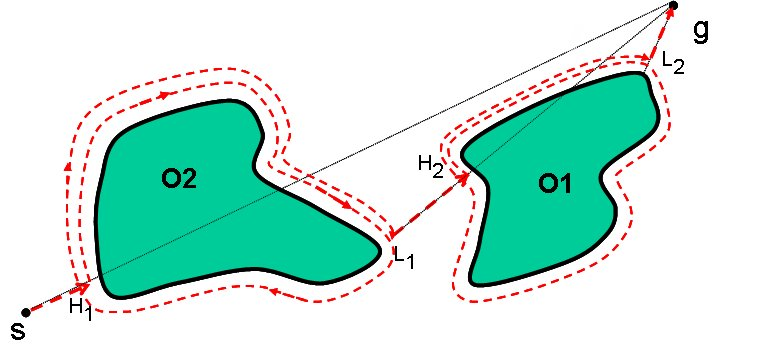
\includegraphics[width=\textwidth]{figures/fig_bug1.png}
        %\caption{Dijkstra}
    }
   \caption[Bug1]{A path created by Bug1 algorithm.(taken from \cite{ribeiro2005obstacle})}
   \label{fig:bug1}
\end{figure}

The Bug2 algorithm tries to immediately change from wall-following to goal-approaching behavior as soon as it encounters a point on the contour which intersects with the straight line connecting starting and goal position, which on average produces shorter paths than Bug1.
Figure~\ref{fig:bug2} shows the Bug2 strategy. 

\begin{figure}[thpb]
	  \myfloatalign
      \footnotesize
      \centering
    \subfloat[]
    {  
        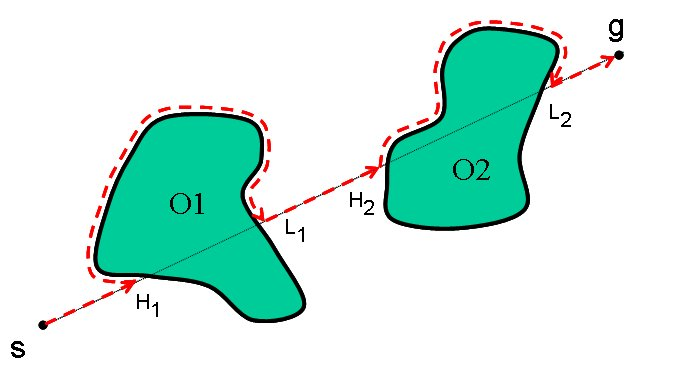
\includegraphics[width=\textwidth]{figures/fig_bug2.png}
        %\caption{Dijkstra}
    }
   \caption[Bug2]{A path created by Bug2 algorithm.(taken from \cite{ribeiro2005obstacle})}
   \label{fig:bug2}
\end{figure}

Many improvements on the original approach are presented in the literature(eg.TangentBug, PointBug, VisBug,...).

\section{Elastic Bands}
Khatib potential field Bubble band

\section{Vector Field Histogram (VFH)}
Vector Field Histograms \cite{borenstein1991vector} simplify the representation of the environment in a 2 step approach to allow for fast calculation of good directions for holonomic robots.
In a first step a small local two-dimensional Cartesian \emph{histogram grid} is created.
Each cell of the grid is incremented if an obstacle is reported from the sensors of the robot. 
Cells with higher values indicate a higher probability of an obstacle at this location, which account for the uncertainty of the sensor readings. 

In a second step the grid is further reduced into a \emph{polar histogram} with angles at the $x$-axis which indicate an obstacle. 
The angles are divided into a discrete set of sectors and each sector obtains an obstacle density value based on the values from the histogram grid.
A threshold value is used to identify valleys in the polar histogram which are used to find gaps large enough for the robot.
The identified valleys are then evaluated using a cost function.
Figure \ref{fig:vfh} shows an example of the resulting diagrams.
\begin{figure}[thpb]
	  \myfloatalign
      \footnotesize
      \centering
    \subfloat[Histogram grid]
    {  
        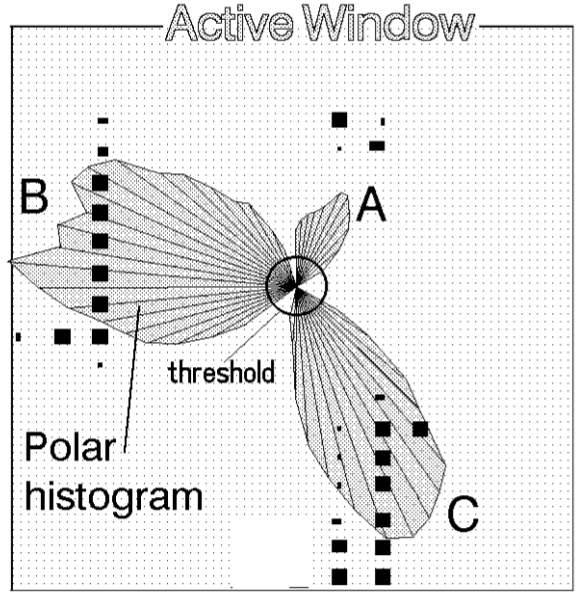
\includegraphics[width=0.75\textwidth]{figures/fig_histogram.png}
        %\caption{Dijkstra}
    }\\
    \subfloat[Polar histogram]
    {  
       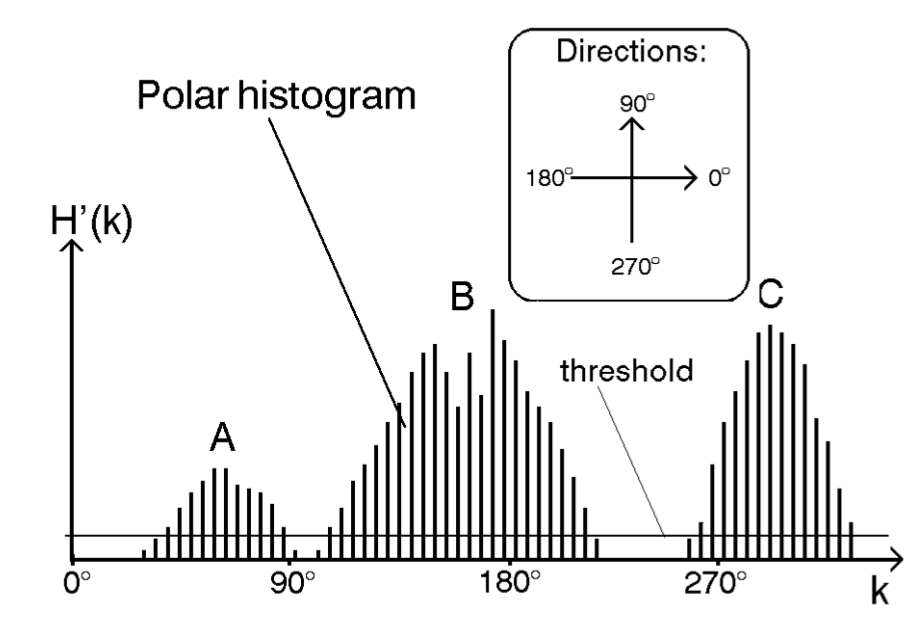
\includegraphics[width=0.75\textwidth]{figures/fig_polar.png}
       %\caption{A*}
    }
   \caption[Vector Field Histogram.]{Figure (a) shows the histogram grid of the Vector Field Histogram method. Figure (b) shows the corresponding polar grid. Large enough gaps in the polar grid are used to find the optimal steering directions for the robot.(taken from \cite{borenstein1991vector})}
   \label{fig:vfh}
\end{figure}

Improvements of this method can be found in the VFH$+$ \cite{ulrich1998vfh+} and VFH$^*$ \cite{ulrich2000vfh} method. 
Here the second step yields an even simpler \emph{binary} polar histogram, where $1$ indicate a blocked and $0$ a free sector. 
In addition some of the kinematics and dynamics are taken into account and the purely local approach is enhanced by adding information of a global path planning component using A$^*$ algorithm. 

\section{Nearness Diagrams (ND)}
Another approach that makes use of graphic representation as a diagram is the Nearness Diagram method presented in \cite{minguez2004nearness} and its refinement in ND+ \cite{minguez2004divide}.
The surrounding of the holonomic robot, approximated as a circle, is divided into a set of different sectors similar to the VFH method.

Sensor information about obstacles is used online to generate two different kind of diagrams.
The PND represents the nearness to obstacles to the center, and the RND the nearness to obstacles to the robots boundary. 
These diagrams are used to categorize different regions in the surrounding of the robot.
RND is used to guarantee safety constraints for the robot, while PND is used to identify valleys which are used for further evaluation.
The region which is closest to the goal and reachable by the robot is selected as the \emph{Free walking area}.
Figure \ref{fig:fig_nd} shows identified regions and the corresponding diagrams.
\begin{figure}[thpb]
	  \myfloatalign
      \footnotesize
      \centering
    \subfloat[Regions in the surrounding of the robot.]
    {  
        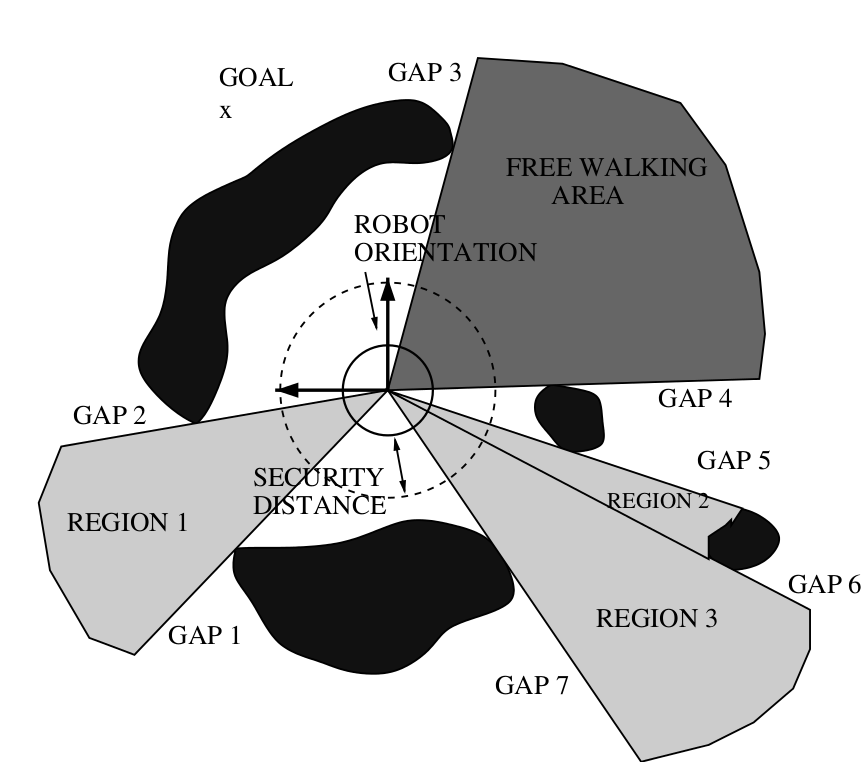
\includegraphics[width=0.75\textwidth]{figures/fig_NDoverview.png}
        %\caption{Dijkstra}
    }\\
    \subfloat[PND diagram]
    {  
       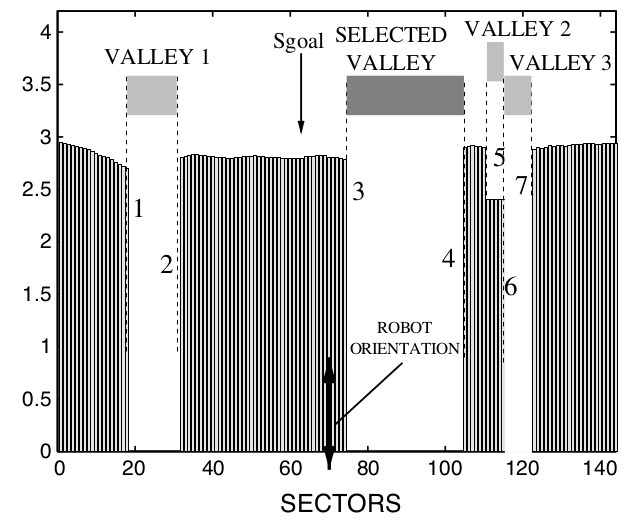
\includegraphics[width=0.5\textwidth]{figures/fig_NDPND.png}
       %\caption{A*}
    }
    \subfloat[RND diagram]
    {  
       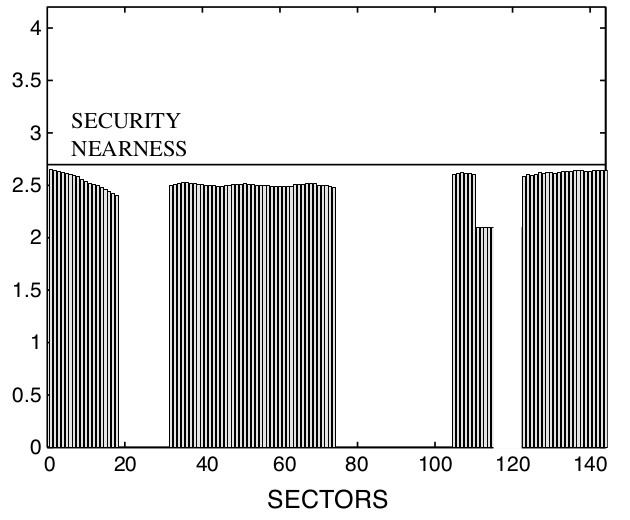
\includegraphics[width=0.5\textwidth]{figures/fig_NDRND.png}
       %\caption{A*}
    }
   \caption[Nearness Diagram.]{Figure (a) shows identified regions using the PND diagram in (b) and RND diagram in (c).(taken from \cite{minguez2004nearness})}
   \label{fig:fig_nd}
\end{figure}

The best actual steering direction is evaluated using a binary decision tree representing a set of predefined \emph{situation} and \emph{action} pairs. 
The values of RND and PND are applied as input and are processed by the branching rules of the tree. 

Improvements to this mehthod are the Generald Nearness Diagrams (GND) method presented in \cite{minguez2001global} which adds global information to the evaluation process. 
The Smooth Nearness Diagrams (SND) introduced in \cite{durham2008smooth} improves on the ND+ method by providing a unique motion law for all situations and incorporating all visible obstacles surrounding the robot, creating smoother paths for the robot.
 
\section{Curvature Velocity Method (CVM)}
The Curvature Velocity Method in \cite{simmons1996curvature} describes an obstacle avoidance method which considers kinematic and dynamic constraints of the robot and the environment.
These constraints are added to a \emph{velocity space} which consists of \emph{translational velocity} $v$ and \emph{rotational velocity} $w$.
One basic assumption of this approach is that the robot can only travel along circles with curvature $c=w/v$. 
This approximation neglects acceleration issues and restricts the robot motions to constant velocities over a given time horizon. 
  
Another simplification is the representation of obstacles as circles, which is used for fast transformation of the obstacles into the velocity space.
All curvatures which do not hit obstacles and adhere to the kinematic constraints of the robot are then evaluated using a cost function.
Since approximation techniques like simulated annealing to maximize the cost function using the whole velocity space did not succeed, the velocity space is divided into finite sets of curvature intervals.
The objective function is then evaluated over all curvature intervals.

A problem of this method arises when confronted with narrow passages which are perpendicular to the robots heading, which might lead to missing shorter paths. 
This problem is solved by the Lane Curvature Method \cite{ko1998lane}, by
dividing the workspace into finite number of lanes. 
The best angular velocity for changing lanes is evaluated using the CVM method. 

\section{Dynamic Window Approach (DWA)}\label{sec:dwa}
A well known method for local planning is the Dynamic Window Approach proposed in \cite{DWA1997}. 
The method samples the \emph{velocity space} $(v,w)$ of the robot, where again $v$ is the \emph{linear velocity} and $w$ the \emph{angular velocity} of the robot, to create a set of feasible trajectories.
The space is reduced to a \emph{dynamic window} which contains the reachable minimal and maximal velocity in one control cycle, taken the acceleration limits of the robot into account.

Obstacles are transformed into the velocity space using a distance function.
Figure \ref{fig:fig_dynamic} shows the obstacles in velocity space and the corresponding dynamic window. 
\begin{figure}[thpb]
	  \myfloatalign
      \scriptsize
      \centering
    \subfloat
    {  
       \def\svgwidth{\textwidth}
       \includesvg{figures/fig_dynamic}
    } 
   \caption[Dynamic Window]{This Figure shows a dynamic window $V_d$ of a robot together with obstacles transformed in a velocity space $V_s$. Only the velocities within the small area around the current robots speed $V_r$ are used for evaluating trajectories by a cost function. The best velocities are forwarded to the robots motor controller. (reproduced from \cite{DWA1997})}
   \label{fig:fig_dynamic}
\end{figure}


For a fixed amount of velocity samples the corresponding trajectories are created using a predefined granularity by performing forward simulation for a short period of time, starting at the current position and speed of the robot. 
The trajectories which stop safely before an obstacles are called \emph{feasible}.
Evaluating all \emph{feasible} trajectories with respect to a weighted cost function (cf. Equation~\ref{eq:costfunction}) identifies the best velocity tuple, which is then forwarded to the motor controller.

\begin{equation}
   f_c(v,w)=\alpha f_a(v,w)+\beta f_d(v,w)+\gamma f_v(v,w)
   \label{eq:costfunction}
\end{equation}

The function $f_a(v,w)$ judges the angle between the robots heading and a given goal position.
It is maximal if the heading is a straight line to the goal.
The distance to the closest obstacle is calculated in the function $f_d(v,w)$.
The function $f_v(v,w)$ takes the forward velocity into account and rewards faster movements of the robot.

In this method the obstacles are not approximated by circles, instead small lines are used to account for a more accurate representation of obstacles.
The robot is still approximated as a circle.
The original method does not use a global plan to guide the robot, so without further changes it is subject to get captured in local minima.

Other applications of this approach in recent planning systems adapt the corresponding cost function. 
%give some recent papers about dwa in developments%
The excellent \texttt{move\_base}\footnote{move\_base planning framework: \url{http://wiki.ros.org/move_base}} motion planning framework introduced in \cite{DBLP:conf/icra/Marder-EppsteinBFGK10} implements within the navigation stack of Robot Operating System (ROS) a local planner which uses a global plan as a guide, and uses a polygon to model the robot outline.

One implementation is based on DWA.
There is also the option to use Trajectory rollout \cite{gerkey08planning} as a local planner which is very related to the DWA, but in contrast improves in simulating the robots trajectory by accurately applying acceleration limits over the whole simulation time.
The cost function maximizes characteristics like proximity to obstacles, proximity to the goal, proximity to the global path, and speed.
Furthermore a number of escaping strategies try to avoid the vulnerability to local minima. 

Collision detection and cost calculation is performed by using the footprint of the robot following the calculated trajectory.
Hence the discretized footprint, which is usually given as a simple polygon, is projected on the costmap. 
Bresenham's Line algorithm \cite{bresenham1965algorithm} is used for ray-tracing the contour of a robot in the discrete workspace. 
Figure~\ref{fig:fig_global} shows the global view of the planning task. 
In Figure~\ref{fig:fig_local} the corresponding local view is depicted, including all sampled trajectories which are evaluated using a local costmap.

\begin{figure}[thpb]
	  \myfloatalign
      \footnotesize
      \centering
    \subfloat[Path planning in global costmap.(taken from \cite{myself})]
    {  \label{fig:fig_global}
       \def\svgwidth{0.75\textwidth}
       \includesvg{figures/fig_global}

    } \\    
    \subfloat[Trajectory generation for linear, and angular velocities $(v,w)$ in local costmap guided by global path.(taken from \cite{myself})]
    {  \label{fig:fig_local}
       \def\svgwidth{0.75\textwidth}
       \includesvg{figures/fig_local}
    }
   \caption[]{}
   \label{fig:fig_dwa}
\end{figure}

Concerning the optimization of the used cost functions the most common approach for DWA and related local planner is to evaluate all possible trajectories in a reduced discrete velocity space. 
Examples of this approach can be found in \cite{kiss2012advanced}\cite{DBLP:conf/icra/Marder-EppsteinBFGK10}\cite{conf/icra/SederP07}. 

The proposed method extends the DWA approach, by using approximation algorithm to maximize the cost function in a discrete representation of the velocity space.

%*****************************************
%*****************************************
%*****************************************
%*****************************************
%*****************************************




